
Para utilizar a ferramenta, o engenheiro de aplica��o deve possuir a especifica��o de requisitos de uma aplica��o em um dom�nio que a ferramenta forne�a apoio, editar os dados dessa especifica��o na ferramenta, gerar artefatos e utilizar esses artefatos no desenvolvimento de aplica��es.

\subsection{Exerc�cio 2 - Utiliza��o da ferramenta}\label{subsec:exercicio2}

O estudo conduzido nesse exerc�cio deve implementar as classes persistentes para as tabelas relacionais apresentadas na Figura \ref{fig:tabelasrelacionais}.

\begin{figure} [!ht]
 \centering
  \bfseries
  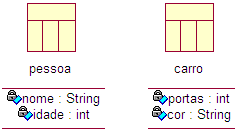
\includegraphics [width=0.45\textwidth]{res/tabelasrelacionais}
  \caption {Tabelas relacionais da aplica��o exemplo}
  \label{fig:tabelasrelacionais}
\end{figure}

As tabelas relacionais apresentadas na Figura \ref{fig:tabelasrelacionais} s�o mapeadas para as classes persistentes apresentadas na Figura \ref{fig:uml}.

\begin{figure} [!ht]
 \centering
  \bfseries
  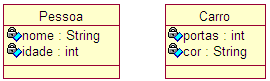
\includegraphics [width=0.45\textwidth]{res/uml}
  \caption {Classes persitentes}
  \label{fig:uml}
\end{figure}

Para o exerc�cio de utiliza��o da ferramenta Captor s�o propostas as seguintes atividades:

\begin{itemize}
	\item Edi��o de uma especifica��o da ferramenta Captor que represente as tabelas e classes apresentadas nas Figuras \ref{fig:tabelasrelacionais} e \ref{fig:uml}.
	\item Gera��o dos artefatos.
	\item Teste dos artefatos gerados.
	\item Cria��o de zonas de seguran�a nos templates para adi��o de novos m�todos nas classes geradas.
	\item Modifica��o dos artefatos gerados dentro das zonas de seguran�a.
\end{itemize}

%------------------------------------------------------------------------------
